\documentclass[a4paper]{article}
\usepackage[left=3cm,right=3cm,top=2cm,bottom=2cm]{geometry} % page settings
\usepackage{enumerate}
\usepackage{hyperref}
\usepackage{graphicx}
\usepackage{amsfonts}
\usepackage{amsthm}
\usepackage{mathtools}
\usepackage{titlesec}
\usepackage{polski}
\usepackage{tikz}
\usepackage[utf8]{inputenc}
\DeclarePairedDelimiter\ceil{\lceil}{\rceil}
\DeclarePairedDelimiter\floor{\lfloor}{\rfloor}

\def\checkmark{\tikz\fill[scale=0.3](0,.35) -- (.25,0) -- (1,.7) -- (.25,.15) -- cycle;} 

\titlespacing*{\subsection}
{0ex}{10ex}{3ex}

\title{Lista 11}
\author{Kamil Matuszewski}
\date{\today}

\begin{document}

\maketitle
\setlength{\parindent}{0.5ex}
\setlength{\parskip}{1.5ex}

\begin{center}
\begin{tabular}{|c *{16}{|c} |c|}\hline
1 & 2 & 3 & 4 & 5 & 6 & 7 & 8 & 9 & 10 & 11 & 12 & 13 & 14 & 15 & 16 & 17 & 18\\
\hline 
\checkmark & \checkmark &  & &  &  & \checkmark & \checkmark & \checkmark & \checkmark &  & \checkmark &  &  &  &  &  & \\
\hline
\end{tabular}\\
\end{center}

\subsection*{Zadanie 1}
Z poprzedniej listy wiemy, że zbiór wierzchołków centralnych drzewa składa się z jednego wierzchołka albo dwóch sąsiednich.\\
Pokażę, że w automorfizmie drzewa centrum zawsze jest punktem stałym automorfizmu.
\begin{proof}
Indukcja po liczbie wierzchołków drzewa. Dla $n={1,2}$ oczywiste. Załóżmy, że dla $\forall k<n$ działa. Sprawdzę dla n.\\
Weźmy dowolne n-wierzchołkowe drzewo. Usuńmy z niego wszystkie liście. Oczywiście operacja usunięcia liści nie zmieniła nam centrum. Skoro tak, to te centrum jest punktem stałym przekształcenia (z zał. ind). Teraz w dowolnym automorfizmie liść musi przechodzić na liść, a jeśli coś jest punktem stałym drzewa, to jest też punktem stałym tego samego drzewa z jakimiś liśćmi. Skoro tak, to centrum drzewa n-wierzchołkowego jest punktem stałym automorfizmu.
\end{proof}
Wiedząc, że w centrum drzewa zawsze jest albo wierzchołek albo para wierzchołków, oraz że centrum drzewa to zawsze punkt stały automorfizmu, widać, że punktem stałym w automorfizmie drzewa jest albo wierzchołek albo krawędź(para wierzchołków).


\subsection*{Zadanie 2}
Gdy n-wierzchołkowy graf G jest samodopełniający, to $n\equiv 0$ lub $n \equiv 1$ modulo 4.
\begin{proof}
Wiemy, że graf jest samodopełniający, gdy jet izomorficzny ze swoim dopełnieniem. Skoro tak, to $G$ ma tyle samo krawędzi co $\widehat{G}$. Poza tym, kiedy zsumujemy graf G ze swoim dopełnieniem, otrzymujemy graf pełny. Wiemy też, że graf pełny ma $\frac{n(n-1)}{2}$ krawędzi.\\
$$\# E(G)+\# E(\widehat{G})=\frac{n(n-1)}{2} \cap \# E(G)=\# E(\widehat{G}) \Rightarrow \# E(G)=\frac{n(n-1)}{4}$$\\
Skoro liczba krawędzi musi być liczbą całkowitą, to albo $n$ jest podzielne na 4, albo $n-1$ jest podzielne na 4 ($NWD(n,n-1)=1$). Czyli $n\equiv 0$ lub $n \equiv 1$ modulo 4.
\end{proof}
\clearpage
Gdy graf G ma n wierzchołków, gdzie $n\equiv 0$ lub $n \equiv 1$ modulo 4, to istnieje graf G który jest samodopełniający.
\begin{proof}
\begin{itemize}
\item $n\equiv 0$ mod $4$\\
Podzielmy n na cztery równoliczne grupy. Nazwijmy te grupy A,B,C i D. Teraz niech każde dwa wierzchołki w A będą połączone krawędzią (podgraf A jest grafem pełnym). Podobnie dla B. Sytuacja odwrotna będzie w C i D (podgrafy C i D są podgrafami pustymi). Teraz każdy wierzchołek z A połączmy z każdym wierzchołkiem z C, każdy wierzchołek C z każdym z D, każdy z D z każdym z B. Twierdzę, ze tak skonstruowany graf jest grafem samodopełniającym.\\
Weźmy dopełnienie stworzonego grafu. W dopełnieniu, krawędzie w A i B znikną, ale pojawią się krawędzie w C i D. Znikną krawędzie między A i C oraz C i D, pojawią się natomiast pomiędzy C i B. Znikną krawędzie pomiędzy D i B pojawią się natomiast pomiędzy D i A. Dodatkowo pojawią się krawędzie pomiędzy A i B. Możemy zauważyć, że A zmieniło się miejscami z D a B z C: podgrafy C i D są podgrafami pełnymi, A i B są podgrafami pustymi. Pomiędzy podgrafami pełnymi nie ma krawędzi, natomiast są krawędzie pomiędzy C i B, B i A, A i D. Możemy więc utworzyć izomorfizm pomiędzy grafem G a jego dopełnieniem.\\
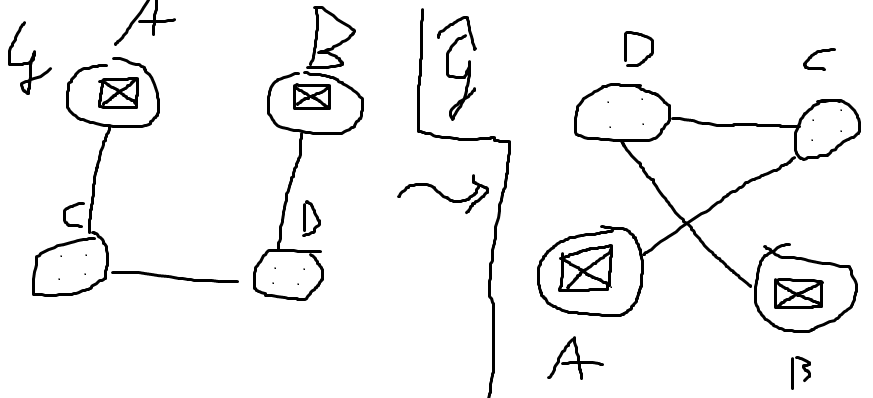
\includegraphics[scale=0.5]{zad2.png}
\item $n\equiv 1$ mod $4$\\
Tutaj konstrukcja jest identyczna do tej w poprzednim przypadku. Zostaje nam jeden wierzchołek, który połączymy ze wszystkimi wierzchołkami z A i B. W dopełnieniu te krawędzie znikną, ale pojawią się krawędzie pomiędzy tym wierzchołkiem a wszystkimi wierzchołkami w C i D. A zmieniło się miejscami z D a B z C, więc nadal istnieje izomorfizm pomiędzy $G$ a $\widehat{G}$.\\
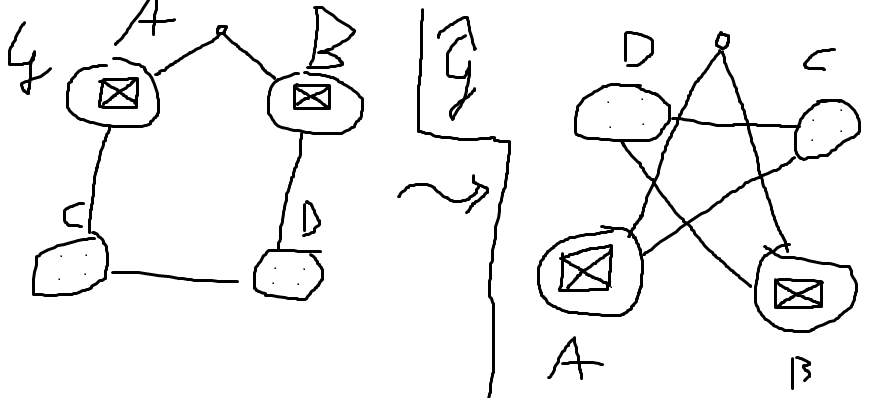
\includegraphics[scale=0.5]{zad2b.png}
\end{itemize}
\end{proof}
\clearpage
\subsection*{Zadanie 7}
W każdym turnieju istnieje wierzchołek, z którego można dojść do każdego innego po drodze skierowanej długości co najwyżej 2.
\begin{proof}
Wieźmy wierzchołek v o największej liczbie łuków wychodzących (maksymalnym $outdeg$). Jeśli $outdeg(v)=\# E(G)$ to z tego wierzchołka istnieje droga do każdego innego o długości dokładnie 1, co kończy zadanie. Załóżmy więc, że $outdeg(v)<\# E(G)$.\\
Załóżmy nie wprost że istnieje wierzchołek u, do którego nie da się dojść ścieżką skierowaną z v w dwóch ruchach. Skoro ten wierzchołek ma łuki do każdego innego wierzchołka, w szczególności ma łuki do wierzchołka v i każdego wierzchołka do którego da się dojść z v w jednym ruchu. Aby nie dało się dojść z v do u w maksymalnie dwóch ruchach, te wierzchołki muszą być połączone krawędziami wychodzącymi z u. Oznacza to, że $outdeg(u)=oustdeg(v)+1$ bo nie dość, że wychodzą z niego krawędzie skierowanie do każdego z $outdeg(v)$ to także wychodzi z niego krawędź skierowana do v. Skoro tak, to nie wybraliśmy wierzchołka o maksymalnej liczbie łuków wychodzących, więc mamy sprzeczność.
\end{proof}

\subsection*{Zadanie 8}
Turniej zawiera drogę Hamiltona.
\begin{proof}
Indukcja. Dla $n=1$ oczywiste, że działa. Zał, że działa dla $n-1$, sprawdzę dla n.\\
Weźmy graf n-wierzchołkowy i usuńmy dowolny wierzchołek u. Oczywiście graf otrzymany po usunięciu tego wierzchołka ma drogę Hamiltona $v_0 \mapsto v_1 \mapsto \cdots \mapsto v_{n-1}$ (zał. indukcyjne). Teraz dołóżmy z powrotem wierzchołek u. Teraz, u ma łuk z każdym innym wierzchołkiem (bo to turniej). Jeśli istnieje krawędź $u \mapsto v_0$ lub $v_{n-1} \mapsto u$ to mamy rozwiązanie. Jeśli nie, to weźmy najmniejsze $i$ takie, że $u \mapsto v_i$. Skoro to najmniejsze takie i, to $v_{i-1} \mapsto u$. Zastąpmy w naszej drodze Hamiltona $v_{i-1}\mapsto v_{i}$ poprzez $v_{i-1}\mapsto u \mapsto v_{i}$. Otrzymaliśmy drogę Hamiltona, i to jest nasze rozwiązanie.
\end{proof}

\subsection*{Zadanie 9}
\begin{itemize}
\item Czy istnieje sposób obejścia szachownicy 5x5 ruchem konika szachowego?
Tak:\\

$
01|24|19|14|03 \\
18|13|02|09|20 \\
23|08|25|04|15 \\
12|17|06|21|10 \\
07|22|11|16|05 \\ 
$

\item Czy istnieje sposób obejścia szachownicy 5x5 ruchem konika szachowego, gdy wymagamy by konik wrócił na to samo pole?
Nie istnieje. Weźmy szachownicę pomalowaną na czarno-biało (tak jak oryginalna szachownica). Łatwo zauważyć, że ruch konia zawsze jest z pola o jednym kolorze na pole o drugim kolorze. Pól do obejścia jest 25. W takim razie jeśli ruszamy z pola czarnego, przy nieparzystej liczbie ruchów trafiamy na pole białe. W 25 ruchu zawsze trafimy na pole białe, a powinniśmy skończyć na polu czarnym. Analogicznie, gdy ruszamy z białego, zawsze skończymy na czarnym. W takim wypadku nie ma opcji byśmy wrócili w to samo miejsce.

\subsection*{Zadanie 10}
Szukaną drogą jest:\\
$
[b, b, a, b, a, a], [b, a, b, b, a, a], [a, b, b, b, a, a], [a, b, b, a, b, a], [a, b, b, a, a, b], [b, a, b, a, a, b], [b, b, a, a, a,b],$\\$ [b, b, a, a, b, a], [b, a, b, a, b, a], [b, a, a, b, b, a], [a, b, a, b, b, a], [a, a, b, b, b, a], [a, a, b, b, a, b], [a, b, a, b,a, b],$\\ $ [b, a, a, b, a, b], [b, a, a, a, b, b] , [a, b, a, a, b, b], [a, a, b, a, b, b], [a, a, a, b, b, b], [a, a, a, b, b, b]]
$

\subsection*{Zadanie 11}
$
[[c, b, c, c, c, a], [c, c, b, c, c, a], [c, c, c, b, c, a], [c, c, c, c, b, a], [c, c, c, c, a, b], [c, c, c, a, c, b], [c, c, a, c, c, b],$\\ $ [c,a, c, c, c, b], [a, c, c, c, c, b], [a, c, c, c, b, c], [c, a, c, c, b, c], [c, c, a, c, b, c], [c, c, c, a, b, c], [c, c, c, b, a, c],$\\ $ [c, c, b,c, a, c], [c, b, c, c, a, c], [b, c, c, c, a, c], [b, c, c, a, c, c], [c, b, c, a, c, c], [c, c, b, a, c, c], [c, c, a, b, c, c], [c, a, c, b, c,c],$\\ $ [a, c, c, b, c, c], [a, c, b, c, c, c], [c, a, b, c, c, c], [c, b, a, c, c, c], [b, c, a, c, c, c], [b, a, c, c, c, c], [a, b, c, c, c, c],[a, b, c, c, c, c]]
$
\subsection*{Zadanie 12}
Pokaż, że w grafie prostym G, w którym dla dowolnych u,v,w istnieją co najmniej dwie spośród trzech krawędzi $\lbrace u,v \rbrace , \lbrace u,w \rbrace , \lbrace v,w \rbrace $,istnieje cykl Hamiltona.
\begin{proof}
Z twierdzenia Orego, jeśli dla dowolnych u,v niepołączonych bezpośrednio $deg(u)+deg(v)\geq n$ to w G istnieje cykl Hamiltona.\\
W grafie pełnym-trywialne.
Weźmy dowolny n-wierzchołkowy graf G. Teraz weźmy dowolnie dwie krawędzie u,v niepołączone bezpośrednio. Zostaje nam $n-2$ wierzchołki. Weźmy dowolny z tych wierzchołków i nazwijmy go w. Wiemy, że dla pary u,v,w muszą istnieć przynajmniej dwie spośród trzech krawędzi $\lbrace u,v \rbrace , \lbrace u,w \rbrace , \lbrace v,w \rbrace $. Skoro nie ma krawędzi $\lbrace u,v \rbrace$, to v musi być połączony z w i u musi być połączony z w. Wierzchołek w wybraliśmy dowolnie, skoro tak, to v jest połączony z każdym z $n-2$ wierzchołków, podobnie u. Mamy więc $$ deg(u)=deg(v)=n-2 $$ $$deg(u)+deg(v)=2n-4\geq n $$ Więc z twierdzenia Orego, istnieje cykl Hamiltona.

\end{proof}

\end{itemize}

\end{document}
